\documentclass[a4paper]{article}
\usepackage[utf8]{inputenc}
\usepackage[spanish, es-tabla, es-noshorthands]{babel}
\usepackage[table,xcdraw]{xcolor}
\usepackage[a4paper, footnotesep = 1cm, width=20cm, top=2.5cm, height=25cm, textwidth=18cm, textheight=25cm]{geometry}
%\geometry{showframe}

\usepackage{tikz}
\usepackage{amsmath}
\usepackage{amsfonts}
\usepackage{amssymb}
\usepackage{float}
\usepackage{graphicx}
\usepackage{caption}
\usepackage{subcaption}
\usepackage{multicol}
\usepackage{multirow}
\setlength{\doublerulesep}{\arrayrulewidth}
\usepackage{booktabs}
\usepackage{mathrsfs,amsmath}
\usepackage{hyperref}
\hypersetup{
    colorlinks=true,
    linkcolor=blue,
    filecolor=magenta,      
    urlcolor=blue,
    citecolor=blue,    
}

\newcommand{\quotes}[1]{``#1''}
\usepackage{array}
\newcolumntype{C}[1]{>{\centering\let\newline\\\arraybackslash\hspace{0pt}}m{#1}}
\usepackage[american]{circuitikz}
\usetikzlibrary{calc}
\usepackage{fancyhdr}
\usepackage{units} 

\graphicspath{./Imagenes}

\pagestyle{fancy}
\fancyhf{}
\lhead{22.05 ASSD}
\rhead{Mechoulam, Lambertucci, Rodriguez, Londero}
\rfoot{Página \thepage}

\begin{document}
\section{Simulaciones Básicas}

\subsubsection{Simulaciones con Python}
Se utilizó el framework de \textit{GNURadio} para programar cada módulo del sistema encerrado en una interfaz gráfica. Esta interfaz tiene la posibilidad de visualizar al mismo tiempo tanto la señal en tiempo como su espectro en cada nodo del sistema. Se puede elegir entre señales sinusoidales, triangulares, 3/2 seno o moduladas AM como entrada.

\subsubsection{Simulaciones con LTSpice}
Para ambos sistemas, tanto con la llave analógica seleccionada como para el Sample and Hold elegido, se realizaron las correspondientes simulaciones con las exitaciones deseadas, obteniendo así los resultados presentados a continuación.

\textcolor{red}{\textbf{Aclarar bajo qué condiciones, es el punto 6a.}}

max lf398 vin = $\pm 18 \ V$
max 4066 vin = $\pm 7.5 \ V$

\begin{figure}[H]
\centering
\begin{subfigure}{.49\textwidth}
	\centering
	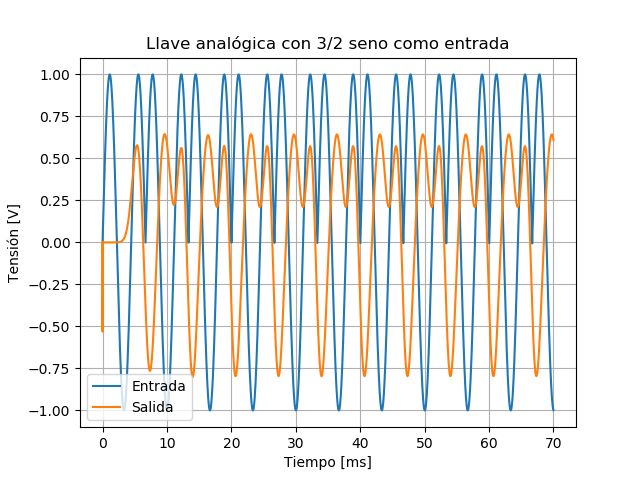
\includegraphics[width=\textwidth]{ImagenesEjercicio6/LA - 3 2.png}
\end{subfigure}
\begin{subfigure}{.49\textwidth}
	\centering
	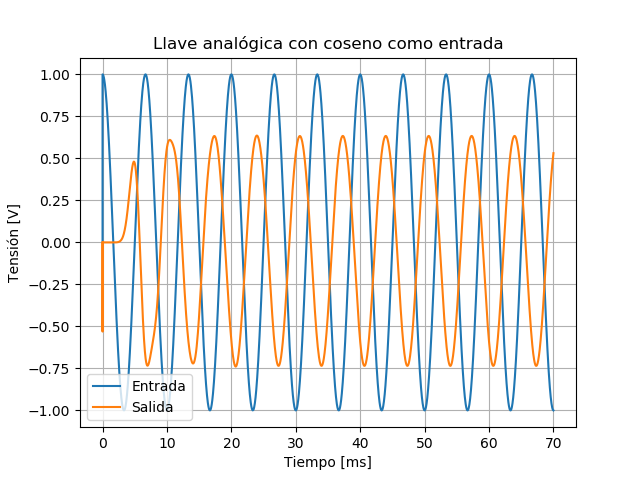
\includegraphics[width=\textwidth]{ImagenesEjercicio6/LA - Cos.png}
\end{subfigure}
\end{figure}
\begin{figure}[H]
\centering
\begin{subfigure}{.49\textwidth}
	\centering
	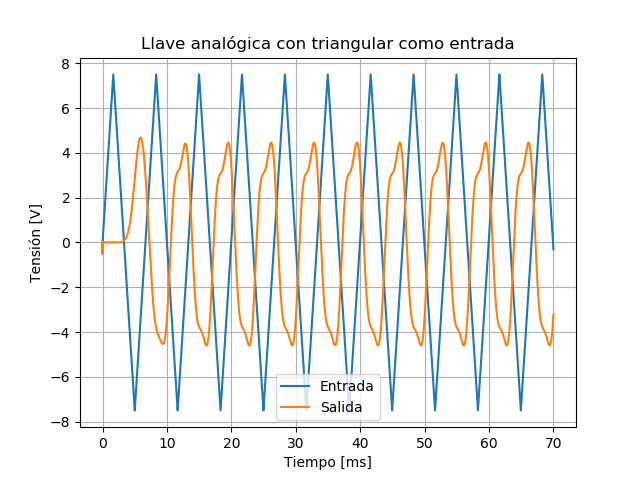
\includegraphics[width=\textwidth]{ImagenesEjercicio6/LA - Tri.png}
\end{subfigure}
\begin{subfigure}{.49\textwidth}
	\centering
	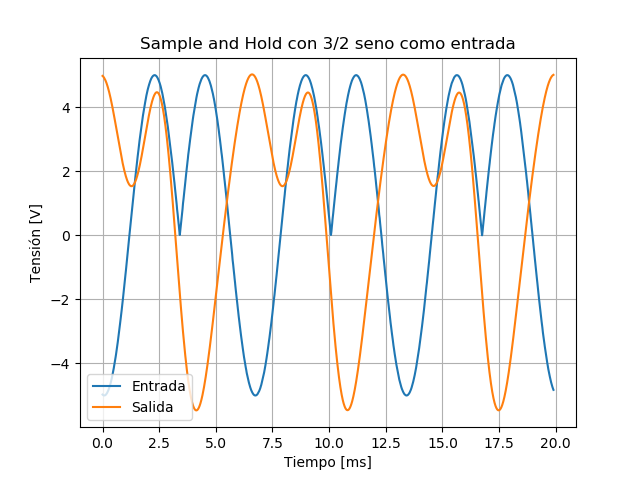
\includegraphics[width=\textwidth]{ImagenesEjercicio6/SH - 3 2.png}
\end{subfigure}
\end{figure}
\begin{figure}[H]
\centering
\begin{subfigure}{.49\textwidth}
	\centering
	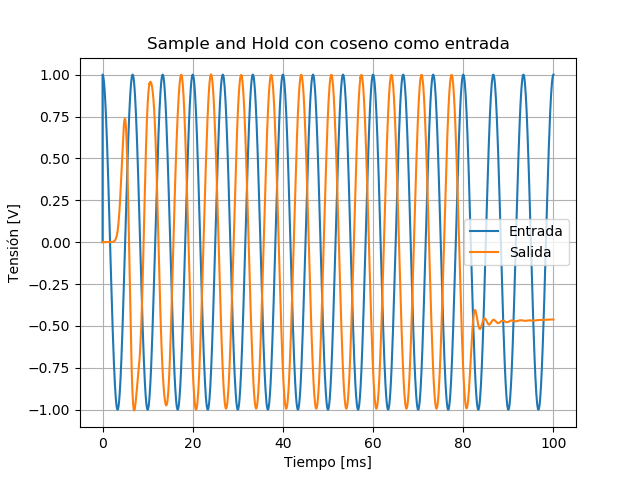
\includegraphics[width=\textwidth]{ImagenesEjercicio6/SH - Cos.png}
\end{subfigure}
\begin{subfigure}{.49\textwidth}
	\centering
	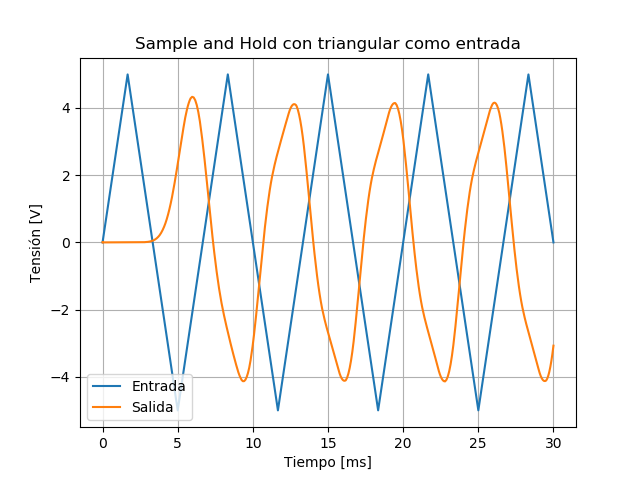
\includegraphics[width=\textwidth]{ImagenesEjercicio6/SH - Tri.png}
\end{subfigure}
\end{figure} 

Nuevamente, se realizaron las mismas simulaciones variando...

\textcolor{red}{\textbf{Aclarar bajo qué condiciones, es el punto 6b.}}



\end{document}